\section{Results}

All times are medians of the measured samples (IQR in parentheses where shown); the full data are in \texttt{results/}. Every run listed here passed its validation
(all $310$ completed process runs have \texttt{correctness = pass}; the three dense timeouts and the five \emph{not attempted} rows have no result to validate), and
all $69$ groups of runs of the same input produced the same SHA-256 of the dense-form product regardless of method or tile size (H3 supported).

\subsection{Part A: dense methods}

\begin{table}[H]
\centering\scriptsize
\begin{tabular}{rrrrrrr}
\toprule
$n$ & i-j-k & i-k-j & blocked & $S_{ikj}$ & $S_{blk}$ & reps \\
\midrule
100 & 0.00112 (0.000223) & 0.000663 (0.0000583) & 0.000768 (0.0000516) & 1.69 & 1.46 & 10/10/10 \\
250 & 0.0176 (0.00167) & 0.0107 (0.00248) & 0.0108 (0.00147) & 1.64 & 1.63 & 10/10/10 \\
500 & 0.162 (0.0160) & 0.112 (0.0296) & 0.106 (0.0485) & 1.45 & 1.53 & 10/10/10 \\
512 & 0.289 (0.0228) & 0.0908 (0.00577) & 0.0990 (0.0212) & 3.18 & 2.91 & 10/10/10 \\
750 & 0.537 (0.0248) & 0.270 (0.0179) & 0.285 (0.0104) & 1.99 & 1.88 & 5/10/10 \\
1000 & 1.60 (0.0989) & 0.690 (0.0320) & 0.695 (0.0955) & 2.32 & 2.30 & 5/10/10 \\
1024 & 3.74 (0.0210) & 0.797 (0.0567) & 0.793 (0.112) & 4.69 & 4.71 & 5/10/10 \\
1250 & 6.50 (0.327) & 1.64 (0.0453) & 1.48 (0.0796) & 3.96 & 4.39 & 5/5/5 \\
2000 & 37.1 (0.333) & 9.95 (0.186) & 6.00 (0.132) & 3.73 & 6.18 & 3/5/5 \\
2048 & 68.4 (4.34) & 9.96 (0.191) & 6.91 (0.499) & 6.87 & 9.89 & 3/5/5 \\
3000 & 190 (0.0805) & 32.6 (0.739) & 21.1 (0.0891) & 5.83 & 8.99 & 2/3/5 \\
4000 & \emph{timeout} & 71.3 (2.70) & 45.4 (1.71) & -- & -- & -/3/3 \\
5000 & \emph{n/a} & 140 (3.00) & 92.8 (1.26) & -- & -- & -/2/3 \\
6000 & \emph{n/a} & 253 (3.55) & 183 (1.61) & -- & -- & -/2/2 \\
8000 & \emph{n/a} & \emph{timeout} & \emph{timeout} & -- & -- & -/-/- \\
\bottomrule
\end{tabular}

\caption{Median time of one multiplication in seconds (IQR in parentheses) of the three dense methods in C, and speed-up over the baseline, $S=t_{ijk}/t$. Reps = number of measured samples for i-j-k / i-k-j / blocked.
Sizes $4000$--$6000$ (i-k-j, blocked only) are listed in Table~\ref{tab:limits}.}
\label{tab:dense}
\end{table}

\begin{figure}[H]
\centering
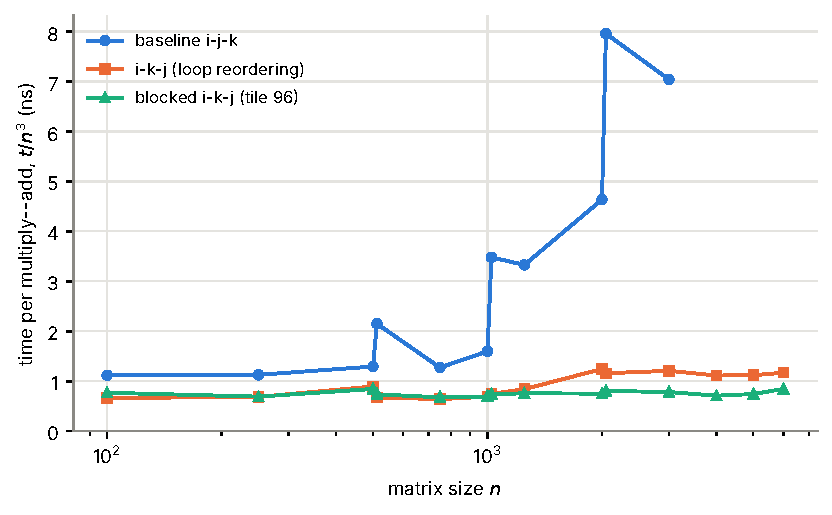
\includegraphics[width=.8\textwidth]{../figures/fig2_dense_normalised.pdf}
\caption{Time per multiply--add, $t/n^3$, against $n$ (median; the IQR is smaller than the markers except at a few sizes, see Table~\ref{tab:dense}).}
\label{fig:norm}
\end{figure}

\paragraph{Loop reordering and blocking.} The baseline costs $1.1$--$1.6$\,ns per multiply--add for $n\le1000$ except at $n=512$ ($2.15$\,ns), and then rises to
$3.5$\,ns at $1024$, $3.3$ at $1250$, $4.6$ at $2000$, $8.0$ at $2048$ and $7.0$ at $3000$ (Figure~\ref{fig:norm}), as in Assignment~1. i-k-j costs $0.64$--$0.89$\,ns up to $n=1250$ and
$1.1$--$1.24$\,ns from $n=2000$; it shows \emph{no} spike at $512$ or $1024$. The blocked method stays between $0.68$ and $0.85$\,ns at \emph{all} sizes up to $6000$.
The speed-up of i-k-j over the baseline is $1.45$--$1.69\times$ for $n\le500$, $2.0$--$2.3\times$ at $750$ and $1000$, and $3.7$--$6.9\times$ for $n\ge1024$ (Figure~\ref{fig:speed});
for the blocked method it is $9.9\times$ at $2048$ and $9.0\times$ at $3000$. The speed-ups are not monotonic in $n$ because the \emph{baseline} is the irregular series:
the largest values ($3.2\times$ at $512$, $4.7\times$ at $1024$, $6.9\times$ and $9.9\times$ at $2048$) coincide with sizes where the baseline itself is anomalously slow, so they partly measure that anomaly.
The blocked method is not faster than i-k-j for $n\le1000$ ($1.00\times$ at $1000$) and gains $1.11\times$ at $1250$, $1.66\times$ at $2000$, $1.44\times$ at $2048$, $1.54\times$ at $3000$, $1.57\times$ at $4000$, $1.51\times$ at $5000$ and $1.38\times$ at $6000$.

\begin{figure}[H]
\centering
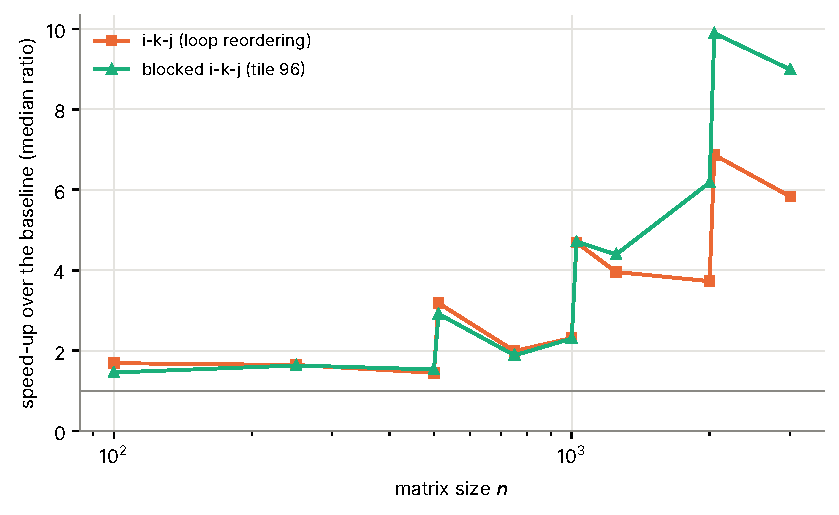
\includegraphics[width=.8\textwidth]{../figures/fig3_dense_speedup.pdf}
\caption{Speed-up over the i-j-k baseline (median ratio). The baseline is measured with only $2$--$5$ samples for $n\ge750$.}
\label{fig:speed}
\end{figure}

\paragraph{Empirical exponents.} Fitting $t\propto n^k$ by least squares in log--log (Table~\ref{tab:fit}; $\pm$ is the $95\%$ confidence interval of the slope, few points, so it is rough):
the blocked method has $k=3.04\pm0.07$ over all feasible $n\ge1000$ (nine sizes), i-k-j $3.26\pm0.19$, and the baseline $4.1\pm1.0$ over $1000$--$3000$ (six points that include the spikes).

\begin{table}[H]
\centering\small
\begin{tabular}{lccc}
\toprule
Method & $n=100$--$500$ & $n=1000$--$3000$ & $n\ge1000$ (all feasible) \\
\midrule
baseline i-j-k & $3.09 \pm 0.68$ (3) & $4.11 \pm 0.97$ (6) & $4.11 \pm 0.97$ (6) \\
i-k-j (loop reordering) & $3.18 \pm 1.23$ (3) & $3.56 \pm 0.28$ (6) & $3.26 \pm 0.19$ (9) \\
blocked i-k-j (tile 96) & $3.05 \pm 1.45$ (3) & $3.09 \pm 0.10$ (6) & $3.04 \pm 0.07$ (9) \\
\bottomrule
\end{tabular}

\caption{Fitted exponent $k$ of $t\propto n^k$ with the $95\%$ CI of the slope and the number of points.}
\label{tab:fit}
\end{table}

\paragraph{Largest feasible size, budget and memory.}
\begin{table}[H]
\centering\scriptsize
\resizebox{\textwidth}{!}{\begin{tabular}{lrrlrrl}
\toprule
Method & Largest feasible $n$ & Largest attempted $n$ & Failures (limit 300 s) & Time at largest ok (s) & Reps & Not attempted \\
\midrule
baseline i-j-k & 3000 & 4000 & 4000: timeout & 190 & 2 & 5000, 6000, 8000 \\
i-k-j (loop reordering) & 6000 & 8000 & 8000: timeout & 253 & 2 & none \\
blocked i-k-j (tile 96) & 6000 & 8000 & 8000: timeout & 183 & 2 & none \\
\bottomrule
\end{tabular}
}
\caption{Largest feasible and largest attempted size under the budgets (300\,s per sample, 4\,GiB). \emph{Not attempted}: skipped after an earlier timeout of the same series.}
\label{tab:limits}
\end{table}
The baseline completes $n=3000$ ($190$\,s) and times out at $4000$; i-k-j and blocked complete $6000$ ($253$\,s and $183$\,s, two samples each) and time out at $8000$.
All limits are set by \emph{time}, not by memory: the largest dense run used $826$\,MiB (Table~\ref{tab:mem}). Peak RSS grows by $24.00$ bytes per $n^2$ in all three methods (three \texttt{float64} matrices, H6)
above a baseline of about $2$\,MiB, and equals the $24n^2$ model within $0.3\%$ at the largest size.

\begin{table}[H]
\centering\scriptsize
\resizebox{\textwidth}{!}{\begin{tabular}{lrrrrr}
\toprule
Method & Peak RSS at $n=100$ (MiB) & Growth (bytes per $n^2$, $n\ge1000$) & Largest $n$ & Peak RSS there (MiB) & $24n^2$ model (MiB) \\
\midrule
baseline i-j-k & 2.00 & 24.00 & 3000 & 207.8 & 206.0 \\
i-k-j (loop reordering) & 2.00 & 24.00 & 6000 & 825.8 & 824.0 \\
blocked i-k-j (tile 96) & 2.00 & 24.00 & 6000 & 825.8 & 824.0 \\
\bottomrule
\end{tabular}
}
\caption{Peak resident memory of the dense methods (\texttt{VmHWM}) and the model $24n^2$ bytes.}
\label{tab:mem}
\end{table}

\paragraph{Bottleneck.} At $n\ge2000$ the baseline spends $4.6$--$8.0$\,ns per multiply--add, $4$--$12$ times the $0.64$--$0.89$\,ns of the unit-stride methods, i.e.\ most of its time is memory access and not arithmetic.
For the unit-stride methods the cost rises from about $0.7$ to $1.1$--$1.2$\,ns for i-k-j when the matrices no longer fit in the caches ($n\ge2000$: $B$ alone is $32$\,MB, much larger than the $1$\,MiB L2), while blocking holds $0.7$--$0.85$\,ns. This is consistent with a cache-capacity effect but, since no hardware counters
are available in the virtual machine, it is an \emph{interpretation}, not a measurement.

\subsection{Tile size, compiler options and variability (supplementary, kept separate)}
\label{sec:resbs}
\begin{table}[H]
\centering\small
\begin{tabular}{rrrrr}
\toprule
Tile $b$ & Process 1 (s) & Process 2 (s) & Mean (s) & $3\cdot8b^2$ (KiB) \\
\midrule
8 & 2.76 & 2.98 & 2.87 & 1.50 \\
16 & 2.54 & 2.77 & 2.65 & 6.00 \\
24 & 2.50 & 2.97 & 2.73 & 13.5 \\
32 & 2.54 & 2.72 & 2.63 & 24.0 \\
48 & 2.76 & 2.75 & 2.76 & 54.0 \\
64 & 2.50 & 2.63 & 2.56 & 96.0 \\
\textbf{96} & 2.47 & 2.53 & \textbf{2.50} & 216 \\
128 & 2.79 & 2.40 & 2.60 & 384 \\
192 & 2.83 & 2.49 & 2.66 & 864 \\
256 & 2.93 & 2.49 & 2.71 & 1536 \\
384 & 2.92 & 2.74 & 2.83 & 3456 \\
\bottomrule
\end{tabular}

\caption{Tile-size sweep of the blocked method at $n=1500$ (seconds, median of two independent processes and their mean). Best tile in bold.}
\label{tab:bs}
\end{table}
The mean time is lowest at $b=96$ ($2.50$\,s), but the whole range $b=16$--$256$ lies within $2.50$--$2.76$\,s ($\le10\%$) and the two processes disagree by up to $0.5$\,s at the same tile size ($b=24$: $2.50$ versus $2.97$\,s); $b=8$ and $b=384$ are $13$--$15\%$ slower.
The landscape is therefore flat and $b=96$ is a reasonable but not a uniquely optimal choice (Figure~\ref{fig:tile}).

\begin{figure}[H]
\centering
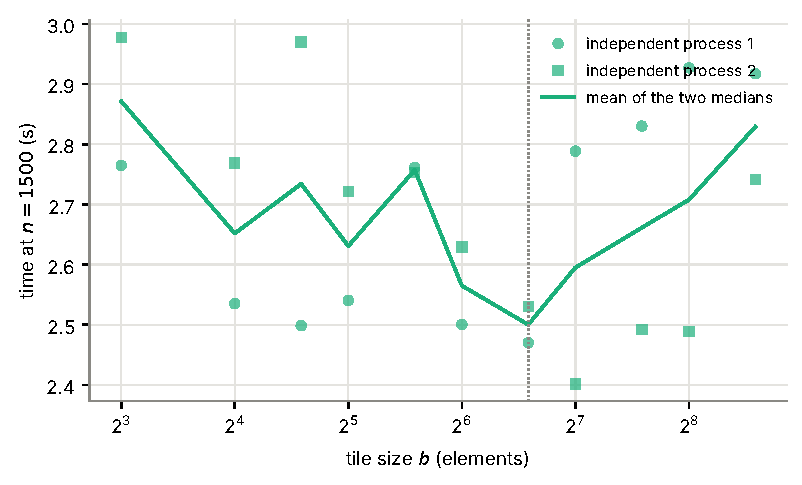
\includegraphics[width=.62\textwidth]{../figures/fig5_tile_sweep.pdf}
\caption{Blocked method at $n=1500$ against the tile size, two processes.}
\label{fig:tile}
\end{figure}

\paragraph{Between-process variability.}\label{sec:resproc} Repeating the same configuration at $n=1000$ in six independent processes (Table~\ref{tab:procvar}) gives medians that differ by $14\%$ (i-k-j), $13\%$ (blocked) and $35\%$ (baseline) from the fastest to the slowest process, which is of the same size as, or larger than,
the within-process IQR ($9$--$14\%$ of the median). Differences between methods or settings below roughly $15\%$ must not be read as real; for the baseline, $35\%$.

\begin{table}[H]
\centering\scriptsize
\begin{tabular}{lrrrrrrrrr}
\toprule
Method & Proc. & P1 (s) & P2 (s) & P3 (s) & P4 (s) & P5 (s) & P6 (s) & Spread (\%) & Within IQR (\%) \\
\midrule
baseline i-j-k & 6 & 1.60 & 1.65 & 2.12 & 1.75 & 1.65 & 1.54 & 35.1 & 9.23 \\
i-k-j (loop reordering) & 6 & 0.690 & 0.724 & 0.753 & 0.795 & 0.738 & 0.728 & 14.3 & 11.1 \\
blocked i-k-j (tile 96) & 6 & 0.695 & 0.758 & 0.775 & 0.789 & 0.734 & 0.752 & 12.5 & 14.0 \\
\bottomrule
\end{tabular}

\caption{Median time at $n=1000$ in six independent processes; spread = (max $-$ min)/min.}
\label{tab:procvar}
\end{table}

\paragraph{Compiler options (Section~\ref{sec:supp}).}
\label{sec:resflags}
\begin{table}[H]
\centering\scriptsize
\begin{tabular}{rlrrrr}
\toprule
$n$ & method & \texttt{-O2} (s) & \texttt{-O2 -funroll-loops} & \texttt{-O3} & \texttt{-O3 -march=native} \\
\midrule
1000 & blocked & 0.865 & 0.495 (1.75$\times$) & 0.242 (3.57$\times$) & 0.232 (3.73$\times$) \\
1000 & ijk & 1.89 & 1.60 (1.18$\times$) & 1.69 (1.11$\times$) & 1.58 (1.19$\times$) \\
1000 & ikj & 0.833 & 0.492 (1.69$\times$) & 0.341 (2.44$\times$) & 0.283 (2.94$\times$) \\
2000 & blocked & 5.99 & 4.02 (1.49$\times$) & 2.59 (2.31$\times$) & 1.83 (3.27$\times$) \\
2000 & ijk & 36.6 & 33.8 (1.08$\times$) & 37.3 (0.98$\times$) & 36.1 (1.02$\times$) \\
2000 & ikj & 9.08 & 8.67 (1.05$\times$) & 6.20 (1.46$\times$) & 5.84 (1.55$\times$) \\
\bottomrule
\end{tabular}

\caption{Median time (s) of each method with other compiler options (in parentheses, speed-up over the same method at \texttt{-O2} in the same experiment; always \texttt{-ffp-contract=off}).}
\label{tab:flags}
\end{table}
At \texttt{-O2} gcc does not vectorise any kernel (no packed multiplication in the object code, \texttt{results/vectorization\_evidence.csv}); at \texttt{-O3} it emits packed multiplications for i-k-j and blocked (128-bit registers; 256-bit with \texttt{-march=native}) and a single one for the baseline, whose inner loop reads a column of $B$ with a stride, and its time does not change. The effect is large:
at $n=1000$ the blocked kernel at \texttt{-O3} is $3.6\times$ faster than at \texttt{-O2}, and at $n=2000$ \texttt{-O3 -march=native} makes blocked $3.3\times$ and i-k-j $1.55\times$ faster, while the baseline does not change ($0.98$--$1.02\times$; the $1.08\times$ of unrolling
is below the variability). The \texttt{-O2} values of this table ($0.83$/$0.87$/$1.89$\,s at $n=1000$) are from a different process than those of Table~\ref{tab:dense} ($0.69$/$0.70$/$1.60$\,s), an instance of the variability above.
The headline comparison of this report uses \texttt{-O2} for all methods; a compiler flag is therefore a larger optimisation than blocking at $n=1000$, and at $n=2000$ it is of the same order.

\subsection{Part B: sparse matrices}

\paragraph{Inputs.} Table~\ref{tab:sparse2000} (and the same tables for $n=500$ and $1000$ in the materials) lists, for each density, the achieved density of the inputs, the density of the product $C$, the CSR kernel time, the separately timed
dense$\to$CSR conversion (both $A$ and $B$), the time of the best dense method of the same cell and of the baseline, and the speed-ups of the CSR kernel $S_k$ and of kernel plus conversion $S_t$ over the best dense method.
Dense times of the same method vary between cells only within the variability above ($0.69$--$0.82$\,s for i-k-j at $n=1000$, $8.4$--$10.1$\,s at $n=2000$, with no trend in density): \emph{the dense methods do not depend on the values}, which also confirms that the comparison base is the same for all densities.

\begin{table}[H]
\centering\scriptsize
\begin{tabular}{lrrrrrrrrr}
\toprule
Input & $d$ (\%) & actual (\%) & $C$ (\%) & CSR kernel (s) & conv. (s) & best dense (s) & i-j-k (s) & $S_k$ & $S_t$ \\
\midrule
random & 0.100 & 0.0998 & 0.199 & 0.000135 & 0.0236 & 5.97 & -- & 44235 & 251 \\
 & 1.00 & 1.00 & 18.2 & 0.0203 & 0.0230 & 6.52 & -- & 322 & 151 \\
 & 5.00 & 5.00 & 99.3 & 0.137 & 0.0303 & 6.59 & -- & 48.2 & 39.4 \\
 & 10.0 & 10.0 & 100 & 0.164 & 0.0315 & 6.26 & -- & 38.3 & 32.1 \\
 & 20.0 & 20.0 & 100 & 0.446 & 0.0448 & 6.11 & -- & 13.7 & 12.4 \\
 & 30.0 & 30.0 & 100 & 1.02 & 0.0558 & 6.04 & -- & 5.95 & 5.64 \\
 & 50.0 & 50.0 & 100 & 3.15 & 0.0741 & 5.84 & 35.8 & 1.86 & 1.81 \\
 & 70.0 & 70.0 & 100 & 5.64 & 0.0715 & 6.01 & -- & 1.07 & 1.05 \\
 & 90.0 & 90.0 & 100 & 9.44 & 0.0645 & 5.81 & -- & 0.615 & 0.611 \\
\midrule
band & 0.100 & 0.1000 & 0.150 & 0.0000410 & 0.0205 & 5.90 & 35.5 & 143712 & 287 \\
 & 1.00 & 0.998 & 1.94 & 0.00191 & 0.0223 & 6.41 & -- & 3358 & 265 \\
 & 5.00 & 4.99 & 9.80 & 0.0222 & 0.0242 & 5.90 & -- & 265 & 127 \\
 & 10.0 & 9.99 & 19.4 & 0.0839 & 0.0252 & 6.10 & -- & 72.7 & 55.9 \\
 & 20.0 & 20.0 & 37.7 & 0.318 & 0.0274 & 5.84 & -- & 18.4 & 16.9 \\
 & 30.0 & 30.0 & 54.6 & 0.720 & 0.0322 & 6.09 & -- & 8.45 & 8.09 \\
 & 50.0 & 50.0 & 82.8 & 2.03 & 0.0410 & 5.74 & -- & 2.83 & 2.77 \\
 & 70.0 & 70.0 & 99.1 & 4.94 & 0.0437 & 6.18 & -- & 1.25 & 1.24 \\
 & 90.0 & 90.0 & 100 & 9.05 & 0.0486 & 5.81 & -- & 0.643 & 0.639 \\
\bottomrule
\end{tabular}

\caption{$n=2000$: CSR$\times$CSR versus the best dense method (blocked). $d$ = density of the inputs (\% nonzero); ``actual'' = measured; $C$ = density of the product. Times in seconds; ``--'' = not run (baseline only at two cells).
$S_k=t_{dense}/t_{kernel}$, $S_t=t_{dense}/(t_{kernel}+t_{conv})$.}
\label{tab:sparse2000}
\end{table}

\begin{figure}[H]
\centering
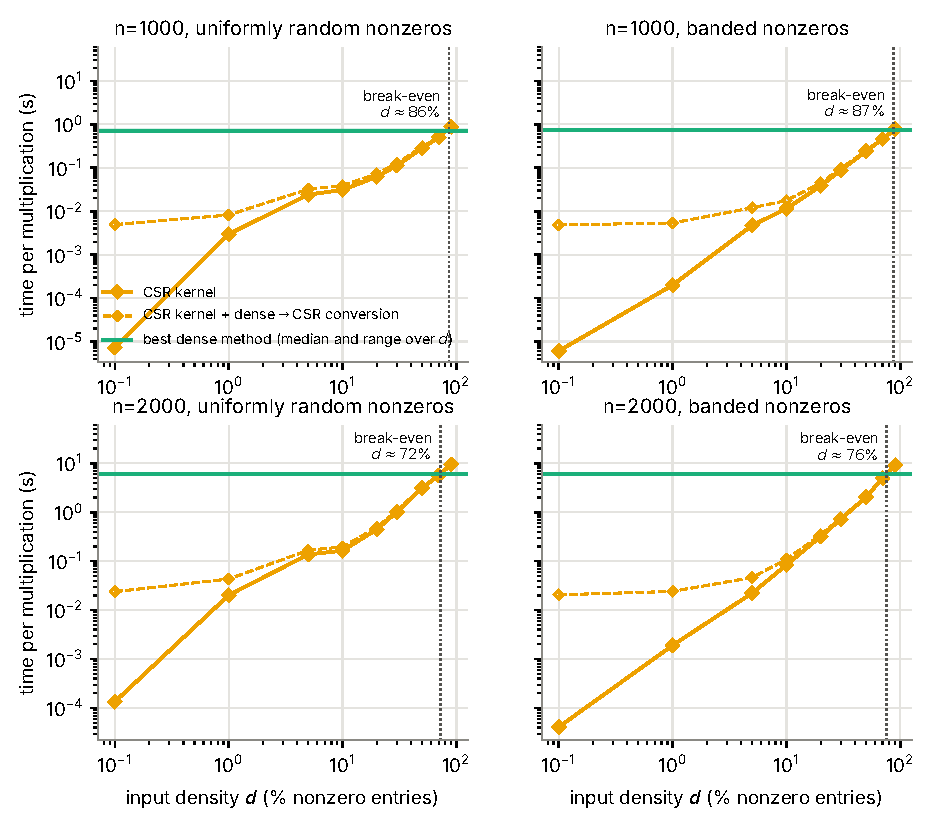
\includegraphics[width=\textwidth]{../figures/fig7_sparse_vs_dense.pdf}
\caption{Time per multiplication of the CSR kernel (with and without the dense$\to$CSR conversion) against the input density $d$. The dense methods do not depend on $d$, so only the best one is drawn: its median over the densities (line) and its range (shaded). The dotted line marks the interpolated break-even density of the kernel. All three dense methods are listed in Table~\ref{tab:sparse2000}.}
\label{fig:sparse}
\end{figure}

\paragraph{Where sparse wins.} At $d=0.1\%$ and $n=1000$ the CSR kernel takes $7.3\,\mu$s (random) and $6.1\,\mu$s (banded), against $0.69$--$0.75$\,s of the best dense method, a ratio of $10^5$; at $n=2000$ the ratios are $4\cdot10^4$ (random) and $1.4\cdot10^5$ (banded).
The advantage falls steadily with density (Figure~\ref{fig:sparse}), is still $1.9$--$3.1\times$ at $d=50\%$ and disappears near the top of the range: the speed-up of the kernel at the largest density tested ($90\%$) is $0.82$--$0.93$ for $n\le1000$ and $0.62$--$0.64$ for $n=2000$; the break-even density, by log--log interpolation
between the neighbouring tested densities, is $82$--$87\%$ for $n=500,1000$ and $72$--$76\%$ for $n=2000$ (\texttt{results/summary\_breakeven.csv}, kernel only; with conversion, $0.2$--$2$ points lower). Because the ratios near $1$ are within the variability ($\pm15\%$), the break-even at $n\le1000$ is only
resolved to about $\pm10$ percentage points; the result at $n=2000$ ($0.61$--$0.64$ at $90\%$) is outside that margin.

\paragraph{Conversion.} Converting two dense matrices to CSR costs $4.8$--$21$\,ms at $n=1000$ and $21$--$74$\,ms at $n=2000$ (it grows with the number of nonzeros, from the minimum at $d=0.1\%$). For $d\le1\%$ banded it is $92$--$99.9\%$ of the end-to-end sparse time (e.g.\ $n=1000$, $d=0.1\%$: kernel $6\,\mu$s, conversion $4.8$\,ms), so the end-to-end advantage is $155\times$ rather than $10^5\times$ (H5 supported);
it falls below $5\%$ of the total for $d\ge70\%$ at $n=1000$ and for $d\ge50\%$ at $n=2000$. If the matrices are already in CSR the conversion does not exist, which is the case of the scaling runs below.

\paragraph{Output density and indexing.} The product of random matrices fills in: at $n=1000$, $C$ has $0.10\%$ of nonzeros for $d=0.1\%$, $9.4\%$ for $d=1\%$, $91.7\%$ for $d=5\%$ and $100\%$ from $d=10\%$, in line with $1-e^{-nd^2}$ ($9.5\%$, $91.8\%$ and $100\%$ predicted) (Figure~\ref{fig:fill}). The product of banded matrices stays banded,
with density $\approx2d$ ($1.9\%$ at $d=1\%$, $19\%$ at $d=10\%$). The cost per useful product of the CSR kernel, $t/\text{flops}$ with flops $=\sum_k\mathrm{colcount}_A(k)\,\mathrm{rowcount}_B(k)$ (Table~\ref{tab:nsflop}), is $0.9$--$1.1$\,ns for banded inputs with $d\ge10\%$ at $n=1000$ (the same order as the dense $0.7$--$0.8$\,ns per
multiply--add) but $30$\,ns for random inputs at $d=1\%$ ($n=1000$) and $25$\,ns at $n=2000$, falling to $9.7$\,ns at $5\%$, $3.1$\,ns at $10\%$ and $1.1$\,ns at $50\%$. In the same density ($1\%$) random and banded inputs differ by $15\times$ in kernel time (3.0\,ms versus 0.20\,ms at $n=1000$) and by $15\times$ in cost per flop.
Hence \emph{the density alone does not determine the performance}: the structure changes the number of useful products, the access pattern to the output workspace, the size of the output and the cost of the column sort. The mechanisms by which random access to a length-$n$ workspace and output growth increase the cost per flop are plausible hypotheses (cache and TLB misses, sorting, \texttt{realloc}), not measured here.

\begin{figure}[H]
\centering
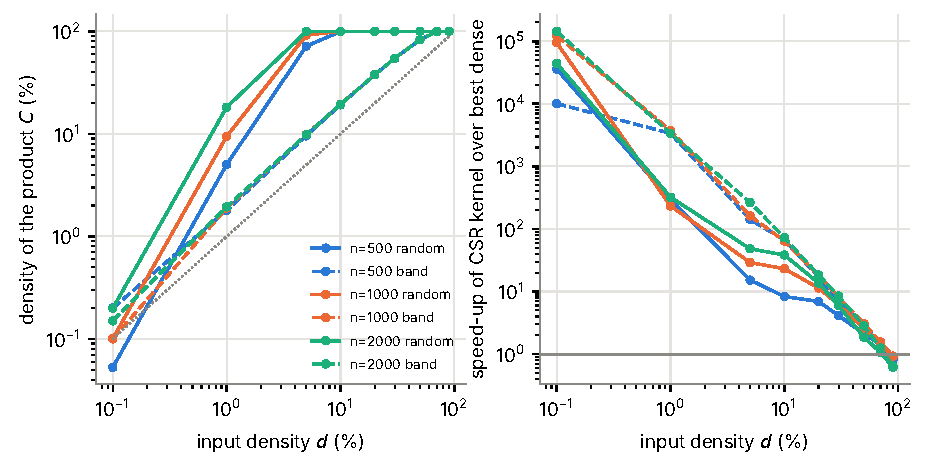
\includegraphics[width=\textwidth]{../figures/fig8_sparse_speedup_output_density.pdf}
\caption{Left: density of the product against input density; the dotted line is $y=x$. Right: speed-up of the CSR kernel over the best dense method (horizontal line: 1).}
\label{fig:fill}
\end{figure}

\begin{table}[H]
\centering\scriptsize
\begin{tabular}{rllrrrr}
\toprule
$n$ & input & $d$ (\%) & $1$ & $5$ & $10$ & $50$ \\
\midrule
1000 & random & ns/flop & 30.0 & 9.66 & 3.13 & 1.12 \\
1000 & banded & ns/flop & 2.00 & 1.87 & 1.13 & 0.93 \\
2000 & random & ns/flop & 25.2 & 6.84 & 2.05 & 1.58 \\
2000 & banded & ns/flop & 2.40 & 1.11 & 1.04 & 0.98 \\
\bottomrule
\end{tabular}
\caption{Cost per useful product of the CSR kernel (ns per flop, flops counted from the CSR operands) at selected densities; the conversion is not included.}
\label{tab:nsflop}
\end{table}

\paragraph{Memory.} The sparse method \emph{csr} holds the dense inputs (to convert them each repetition) and the CSR copies and the output; its peak RSS at $n=2000$ is $63$--$78$\,MiB for $d\le1\%$ but $164$--$200$\,MiB when the product is dense, versus $93$\,MiB for the dense methods (Table~\ref{tab:sparsemem}).
The CSR storage model $12$ bytes per nonzero of $A$, $B$ and $C$ plus $24(n+1)$ matches the measured resident memory of the CSR-only runs (below) within $1\%$ at the sizes with $n\ge32000$ ($d=0.1\%$) and $n\ge8000$ ($d=1\%$).

\begin{table}[H]
\centering\scriptsize
\begin{tabular}{lrrrrr}
\toprule
Input & $d$ (\%) & $C$ (\%) & CSR storage of $A,B,C$ (MiB) & peak RSS sparse (MiB) & peak RSS dense (MiB) \\
\midrule
random & 0.100 & 0.199 & 0.229 & 63.1 & 93.3 \\
 & 1.00 & 18.2 & 9.29 & 78.2 & 93.3 \\
 & 5.00 & 99.3 & 50.1 & 166 & 93.3 \\
 & 10.0 & 100 & 55.0 & 182 & 93.3 \\
 & 20.0 & 100 & 64.1 & 182 & 93.3 \\
 & 30.0 & 100 & 73.3 & 164 & 93.3 \\
 & 50.0 & 100 & 91.6 & 200 & 93.3 \\
 & 70.0 & 100 & 110 & 173 & 93.3 \\
 & 90.0 & 100 & 128 & 191 & 93.3 \\
\midrule
band & 0.100 & 0.150 & 0.206 & 63.0 & 93.3 \\
 & 1.00 & 1.94 & 1.85 & 64.7 & 93.3 \\
 & 5.00 & 9.80 & 9.10 & 71.9 & 93.3 \\
 & 10.0 & 19.4 & 18.1 & 80.9 & 93.3 \\
 & 20.0 & 37.7 & 35.6 & 98.4 & 93.3 \\
 & 30.0 & 54.6 & 52.5 & 115 & 93.3 \\
 & 50.0 & 82.8 & 83.8 & 147 & 93.3 \\
 & 70.0 & 99.1 & 109 & 172 & 93.3 \\
 & 90.0 & 100 & 128 & 191 & 93.3 \\
\bottomrule
\end{tabular}

\caption{$n=2000$: CSR storage of $A$, $B$, $C$ (model) and peak RSS of the \emph{csr} method (dense inputs resident) and of the dense methods.}
\label{tab:sparsemem}
\end{table}

\paragraph{Scaling with CSR inputs and the budget.} With inputs already in CSR (random, \emph{csrfile}) the sizes of Table~\ref{tab:scale} were run. At $d=0.1\%$ the sequence reached $n=64000$ ($14$\,s, $2.9$\,GiB, product density $6.2\%$, $254$ million nonzeros); at $d=1\%$ it reached $n=16000$ ($4.3$\,s, $2.3$\,GiB, product density $80\%$).
The next sizes ($n=128000$ at $0.1\%$, $n=32000$ at $1\%$) were \emph{not attempted} because the predicted memory ($47.6$ and $23.8$\,GB) is more than three times the budget: \textbf{no sparse run hit a real failure}; the limit reported is the largest feasible size, and the next size is excluded by prediction, not by an observed failure.
The time grows as $n^{3.4}$ at $d=0.1\%$ and $n^{2.6}$ at $d=1\%$ over the measured sizes, while the number of useful products grows as $n^{3.0}$ at fixed density, so the cost per flop is not constant ($15$--$69$\,ns at $0.1\%$, $10$--$26$\,ns at $1\%$); memory is dominated by the output, which grows faster than the inputs ($\propto n^{2.5}$ at the largest sizes) because of the fill-in.
For comparison, a dense $n=64000$ product would need $24n^2=98$\,GB (computed, not measured), and the dense methods stopped at $6000$ because of time.

\begin{table}[H]
\centering\scriptsize
\begin{tabular}{rrrrrrrrr}
\toprule
$d$ (\%) & $n$ & nnz($A$) & nnz($C$) & $C$ dens. (\%) & time (s) & reps & peak RSS (MiB) & CSR est. (MiB) \\
\midrule
0.100 & 2000 & 3.99e+03 & 7.97e+03 & 0.199 & 0.000119 & 10 & 2.023 & 0.2286 \\
 & 4000 & 1.63e+04 & 6.52e+04 & 0.407 & 0.00192 & 10 & 4.145 & 1.207 \\
 & 8000 & 6.41e+04 & 5.09e+05 & 0.796 & 0.0295 & 10 & 13.75 & 7.476 \\
 & 16000 & 2.57e+05 & 4.09e+06 & 1.60 & 0.278 & 10 & 96.10 & 52.99 \\
 & 32000 & 1.02e+06 & 3.22e+07 & 3.14 & 2.26 & 5 & 394.6 & 392.5 \\
 & 64000 & 4.1e+06 & 2.54e+08 & 6.20 & 14.0 & 5 & 3004 & 3002 \\
 & 128000 & -- & -- & -- & \emph{not attempted} & -- & -- & -- \\
\midrule
1.00 & 2000 & 4e+04 & 7.28e+05 & 18.2 & 0.0205 & 10 & 17.21 & 9.292 \\
 & 4000 & 1.6e+05 & 5.26e+06 & 32.9 & 0.109 & 10 & 65.84 & 64.00 \\
 & 8000 & 6.39e+05 & 3.52e+07 & 55.1 & 0.811 & 5 & 420.0 & 418.1 \\
 & 16000 & 2.56e+06 & 2.04e+08 & 79.8 & 4.29 & 5 & 2398 & 2396 \\
 & 32000 & -- & -- & -- & \emph{not attempted} & -- & -- & -- \\
\bottomrule
\end{tabular}

\caption{Scaling of the CSR kernel with CSR inputs (random, $d=0.1\%$ and $1\%$). Time = median of the kernel (conversion not applicable); peak RSS measured; CSR est. = $12(\text{nnz}_A+\text{nnz}_B+\text{nnz}_C)+24(n+1)$ bytes.}
\label{tab:scale}
\end{table}

\begin{figure}[H]
\centering
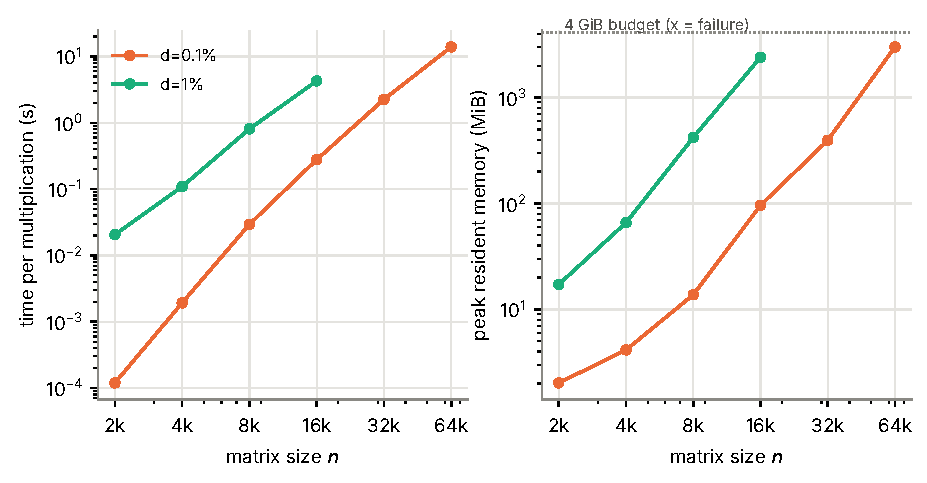
\includegraphics[width=\textwidth]{../figures/fig9_sparse_scaling.pdf}
\caption{Time and peak memory of the CSR kernel against $n$ with CSR inputs. The dotted line is the $4$\,GiB budget; no run failed.}
\label{fig:scale}
\end{figure}

\subsection{Correctness tests}
\begin{table}[H]
\centering\small
\begin{tabular}{lrr}
\toprule
Group of tests & Checks & Passed \\
\midrule
Dense: known answers (scalar, 2$\times$2, 3$\times$3, zero, identity, all-ones, integer) & 117 & 117 \\
Dense: random matrices vs NumPy ($n=5,\dots,129$) & 78 & 78 \\
Dense: bit-for-bit equality of all methods and 13 tile sizes & 13 & 13 \\
Dense: repeated runs give identical checksums & 7 & 7 \\
Sparse: edge cases (empty, identity, diagonal, empty row/column, $1\times1$, fully dense) & 64 & 64 \\
Sparse: random and banded vs SciPy (pattern, values), CSR sorted, csr$=$csrfile & 72 & 72 \\
Sparse: densified result bit-for-bit equal to the dense methods & 24 & 24 \\
Sparse: conversion, spot-check rows, repeated runs & 2 & 2 \\
\midrule
\textbf{Total} & \textbf{377} & \textbf{377} \\
\bottomrule
\end{tabular}

\caption{Results of the correctness suite (run before the benchmarks and again before submission).}
\label{tab:tests}
\end{table}
